\documentclass[journal]{IEEEtran}
\usepackage[T1]{fontenc}
\usepackage[utf8]{inputenc}
\usepackage{amsmath,amssymb,bm}
\usepackage{graphicx,booktabs,array}
\usepackage{cite}
\usepackage{placeins}
\usepackage[hidelinks]{hyperref}
\graphicspath{{figures/}}
\newcommand{\vect}[1]{\mathbf{#1}}
\newcommand{\trans}{^{\mathsf T}}
\newcommand{\norm}[1]{\lVert#1\rVert}
\newcommand{\R}{\mathbb R}
\newcommand{\draftsubsection}[1]{\subsection{#1}\par\penalty0\relax}
\DeclareMathOperator{\diag}{diag}
\DeclareMathOperator{\Var}{Var}
\DeclareMathOperator{\Cov}{Cov}
\begin{document}
\title{Calibration-Aware Three-Dimensional Optical Positioning With a Fixed LED and a Tilt-Constrained Reorientable Photodiode}
\author{Author names and affiliations to be confirmed}
\markboth{IEEE Transactions on Instrumentation and Measurement --- Working Manuscript}{Fixed-LED Positioning With a Reorientable Photodiode}
\maketitle
\begin{abstract}
\end{abstract}
\begin{IEEEkeywords}
\end{IEEEkeywords}

\section{Introduction}
\label{sec:introduction}
\draftsubsection{Background and Motivation}
\draftsubsection{Related Work and Research Gap}
\draftsubsection{Contributions and Organization}

\section{System and Measurement Model}
\label{sec:model}
\subsection{System Geometry}
\label{subsec:geometry}
Consider a fixed LED at a known position $\vect t\in\R^3$, with unit optical axis $\vect n_t$ and constant transmitted power $P_t$. A single PD has an unknown position $\vect r=[x,y,z]\trans$ and acquires RSS measurements at $K$ orientations while its optical center remains stationary. The receiver normals $\vect n_i\in\mathbb S^2$, $i=1,\ldots,K$, are expressed in the same global coordinate frame and may be chosen arbitrarily. All three position coordinates are unknown.

The LED--PD distance and the unit direction from the PD toward the LED are:
\begin{equation}
 d=\norm{\vect t-\vect r},\qquad
 \vect u=\frac{\vect t-\vect r}{d}.
 \label{eq:geometry}
\end{equation}
The irradiance angle $\phi$ and incidence angle $\psi_i$ are determined by:
\begin{equation}
 \cos\phi=-\vect n_t\trans\vect u,\qquad
 \cos\psi_i=\vect n_i\trans\vect u.
 \label{eq:incidence}
\end{equation}
Thus, receiver reorientation changes $\psi_i$, whereas $d$ and $\phi$ remain constant during the acquisition sequence. The inclination of $\vect n_i$ relative to the global vertical is distinct from the incidence angle $\psi_i$; no common inclination or azimuthal spacing is imposed.

\subsection{Received-Power Model}
\label{subsec:radiometry}
Under line-of-sight (LOS) propagation and a Lambertian point-source model~\cite{Kahn1997,Wang2024}, the calibrated received-power observation at orientation $i$ is:
\begin{equation}
 P_{r,i,k}=P_t H_i(\vect r)+\epsilon_{i,k},
 \qquad k=1,\ldots,N_i,
 \label{eq:received-power}
\end{equation}
where $N_i$ is the number of observations, $\epsilon_{i,k}$ is additive noise, and $H_i$ is the effective LOS channel gain:
\begin{equation}
 H_i(\vect r)=\frac{(m_T+1)A_{\mathrm{PD}}}{2\pi d^2}
 \cos^{m_T}(\phi)\,R(\psi_i).
 \label{eq:channel}
\end{equation}
Here $A_{\mathrm{PD}}$ denotes the active detector area. The LED Lambertian order is $m_T=-\ln2/\ln(\cos\Phi_{1/2})$, where $\Phi_{1/2}$ is its semi-angle at half power. Equation~\eqref{eq:channel} applies for $0\leq\phi<\pi/2$ and $0\leq\psi_i<\Psi_{\mathrm{FOV}}\leq\pi/2$; otherwise, $H_i=0$. The receiver FOV is a half-angle. No optical concentrator is assumed, and the on-axis optical transmission is taken as unity. Received powers are expressed in optical-equivalent watts after background removal and gain/responsivity calibration.

\subsection{Receiver Angular Response}
\label{subsec:response}
The dimensionless function $R(\psi)$ describes the normalized effective angular response, with $R(0)=1$. It includes the projected-area effect, so no additional factor $\cos\psi$ is required in~\eqref{eq:channel}. The receiver is assumed to have an axisymmetric response.

The conventional model uses $R(\psi)=\cos\psi$~\cite{Kahn1997,Wang2024}. Experimental characterization of commercial PDs supports alternatives such as $R(\psi)=\cos^{m_R}\psi$, with $m_R>0$, and the SQ model~\cite{Bastiaens2020}:
\begin{equation}
 R_{\mathrm{SQ}}(\psi)=
 \left[1-\frac{1-1/\sqrt2}{\psi_{3\mathrm{dB}}^2}\,\psi^2\right]_+,
 \label{eq:sq-response}
\end{equation}
where $[a]_+=\max(a,0)$ and $\psi_{3\mathrm{dB}}$ is the angle at which the response equals $1/\sqrt2$. The order $m_R$ characterizes the receiver and is independent of $m_T$. The response model and its parameters are determined by calibration; the formulation retains $R(\psi)$ without selecting a particular family. Its response may vanish before the external FOV limit, whereas an angle of half response does not itself define a hard cutoff.

\subsection{RSS Acquisition and Observation Statistics}
\label{subsec:observations}
At each orientation, observations are retained after the receiver has settled, as illustrated in Fig.~\ref{fig:acquisition}. The baseline assumes linear nonsaturated detection and independent Gaussian optical-equivalent noise, $\epsilon_{i,k}\sim\mathcal N(0,\sigma_0^2)$, with calibrated variance $\sigma_0^2$ in $\mathrm W^2$. Defining $\mu_i(\vect r)=P_tH_i(\vect r)$, the averaged observation satisfies:
\begin{equation}
 \bar P_{r,i}=\frac1{N_i}\sum_{k=1}^{N_i}P_{r,i,k}
 \sim\mathcal N\left(\mu_i(\vect r),\frac{\sigma_0^2}{N_i}\right).
 \label{eq:sample-mean}
\end{equation}
The observation vector $\bar{\vect P}_r=[\bar P_{r,1},\ldots,\bar P_{r,K}]\trans$ therefore has covariance:
\begin{equation}
 \bm\Sigma_P=\diag\left(\frac{\sigma_0^2}{N_1},\ldots,
 \frac{\sigma_0^2}{N_K}\right).
 \label{eq:mean-covariance}
\end{equation}
The total sample budget is $M=\sum_i N_i$; increasing $K$ at fixed $N_i$ and at fixed $M$ are different comparisons. The per-observation and averaged-measurement SNRs are:
\begin{equation}
 \mathrm{SNR}_{i,\mathrm{raw}}=\frac{\mu_i^2}{\sigma_0^2},\qquad
 \mathrm{SNR}_{i,\mathrm{mean}}=\frac{N_i\mu_i^2}{\sigma_0^2}.
 \label{eq:snr}
\end{equation}
The actual receiver normals are treated as known in this baseline; orientation uncertainty is introduced in Section~\ref{sec:bounds}. Noise correlation, calibration errors, and deviations from LOS propagation require separate characterization rather than being removed by averaging.

\begin{figure*}[t]
 \centering
 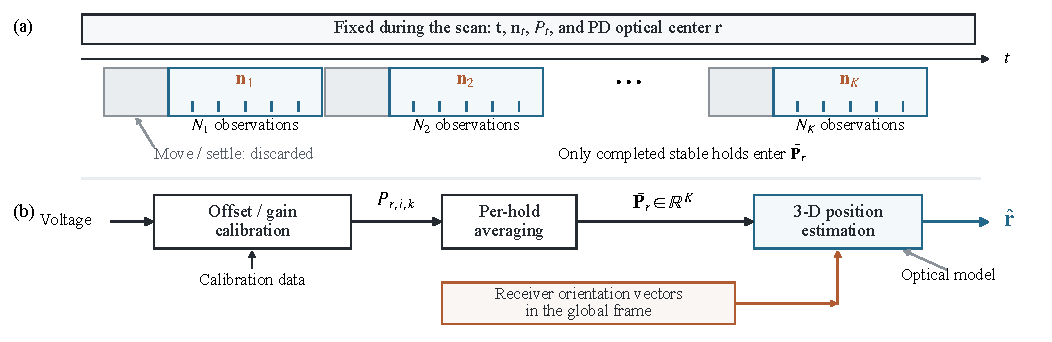
\includegraphics[width=\textwidth]{fig02_acquisition.pdf}
 \caption{Sequential RSS acquisition and processing. Transition intervals are discarded; $N_i$ observations are retained at each stable orientation. Calibrated power means and globally referenced receiver normals form the inputs for position estimation.}
 \label{fig:acquisition}
\end{figure*}

\FloatBarrier

\section{Calibration and Uncertainty Characterization}
\label{sec:calibration}
%\draftsubsection{Radiometric Scale and Transmitter Pattern}
%\draftsubsection{Receiver Angular Response and Model Selection}
%\draftsubsection{Orientation Reference and Optical-Center Calibration}
%\draftsubsection{Noise Statistics, Correlation, and Repeatability}

\section{Identifiability and Position Error Bounds}
\label{sec:bounds}
%\draftsubsection{Local Identifiability and Global Ambiguities}
%\draftsubsection{Fisher Information With Known Orientations}
%\draftsubsection{Effective Information With Orientation Uncertainty}
%\draftsubsection{Position Error Bound and Coverage Criteria}

\section{Estimation and Tilt-Constrained Orientation Design}
\label{sec:estimation}
%\draftsubsection{Estimation With a Calibrated Angular Response}
%\draftsubsection{Cosine-Power Reference Estimators}
%\draftsubsection{Initialization, Model Support, and Failure Detection}
%\draftsubsection{Orientation-Set and Sample-Budget Design}

\section{Experimental Platform and Evaluation Protocol}
\label{sec:experiments}
%\draftsubsection{Optical and Electromechanical Instrumentation}
%\draftsubsection{Position Reference and Its Measurement Uncertainty}
%\draftsubsection{Calibration and Independent Validation Datasets}
%\draftsubsection{Acquisition Procedure, Baselines, and Performance Metrics}

\section{Numerical and Experimental Results}
\label{sec:results}
%\draftsubsection{Three-Dimensional Position Error and Information Bounds}
%\draftsubsection{Inclination, Orientation Count, and Spatial Coverage}
%\draftsubsection{Angular-Response Mismatch and Calibration Sensitivity}
%\draftsubsection{Orientation Errors, Reflections, and Acquisition Time}
%\draftsubsection{Limitations and Transferability}

\section{Conclusion}
\label{sec:conclusion}

\appendices
\section{Channel Derivatives for the Considered Response Families}
\label{app:derivatives}
\section{Estimation and Orientation-Design Procedures}
\label{app:algorithms}

\bibliographystyle{IEEEtran}
\bibliography{references}
\end{document}
